\chapter{ARxCODE}
\label{chap:arxcode} 

%\endinput
\section{Especificaciones generales}

ARxCODE es un prototipo de software dise\~nado para el procesamiento y an\'alisis de encuentros con riesgo de colisi\'on, entre misiones operativas y desechos espaciales.\\
Tiene como objetivo principal procesar la informaci\'on, proveniente de los organismos internacionales de alerta (mensaje CDM), o cargada manualmente, y facilitar al operador la visualizaci\'on de los par\'ametros de la situaci\'on en forma clara para su correcta interpretaci\'on y comunicaci\'on.\\
Es una aplicaci\'on de escritorio, de estructura modular, reusable y modificable que cuenta con una interfaz amigable.\\
Pensada con una filosof\'ia de expansi\'on y perfeccionamiento, su arquitectura permite la adici\'on de funcionalidades sin mayores inconvenientes.\\

% Describir:
% \begin{itemize}
% \itemsep0em
%  \item  M\'odulos Fundamentales.
%  \item Flujo de Pantallas.
%  \item Diagrama de Componentes.
%  \item Requerimientos.
%  \item Casos de USO.
%  \item Entidades (diagrama de clases)
%  \item Diagrama de Secuencia.
%  \item Dise\~no de interfaces.
% \end{itemize}

\section{Requerimientos}\label{sec:requerimientos}

Se pretende que ARxCODE sea una herramienta que oficie de soporte al operador en el di\'alogo con los organismos internacionales que proveen los mensajes de alerta, frente a una situaci\'on de riesgo de colisi\'on. A tal fin, el sistema debe tener la capacidad de interpretar los mensajes estandarizados CDM y presentar la informaci\'on que all\'i se registra, en forma clara al operador.\\
Por otro lado, debe tener la capacidad de colectar datos ingresados manualmente por el operador y ofrecer los par\'ametros que resulten del procesamiento propio del ARxCODE, como m\'inima distancia, TCA calculado y PoC.\\
Esta \'ultima funcionalidad implica que ARxCODE debe poder solicitar a la p\'agina Space-Track los TLEs correspondientes a los objetos involucrados, debe poder estimar las matrices de covarianza de ambos objetos, ya sea mediante el m\'etodo de Osweiler o incorporando efem\'erides predichas del departamento de Din\'amica Orbital; debe poder propagar esos errores al momento del TCA y finalmente calcular la PoC.\\
En la tabla \ref{tab:req}, se listan todos los requerimientos del sistema.\\

\begin{table}[!h]\renewcommand{\arraystretch}{1.15}
 \resizebox{\linewidth}{!}{
 \begin{tabular}{|l|l|}
 \hline \hline 
   \rowcolor{lightgray}
  Req. ID & Descripci\'on \\
  \hline \hline
  \rowcolor{lightgray}
  1 & Requerimientos FUNCIONALES\\
  \hline 
  ARR-010 & ARxCODE debe calcular la probabilidad de colisi\'on de un acercamiento de riesgo.\\
  \hline 
  \multirow{2}{*}{ARR-020} & ARxCODE debe  aceptar como inputs: un mensaje de alerta (CDM), o los identificadores\\
  & de NORAD de ambos objetos y el tiempo de m\'aximo acercamiento (TCA).\\
  \hline 
  \multirow{2}{*}{ARR-030} & ARxCODE debe utilizar los productos orbitales de la misi\'on o realizar el mismo\\
  & procedimiento que se aplica al desecho, a la misi\'on.\\
  \hline 
  ARR-040 & ARxCODE debe calcular la m\'inima distancia, total y en la coordenada radial.\\
  \hline 
  ARR-050 & ARxCODE debe manipular los sistemas de referencia: TEME, TOD y RTN. \\
  \hline
  \multirow{2}{*}{ARR-060}& ARxCODE debe permitir al operador analista experto visualizar el encuentro,\\
  & generar reportes y notificaciones.\\
  \hline
  \multirow{2}{*}{ARR-070} & ARxCODE debe extraer el conjunto de TLEs de los objetos involucrados \\
  & de los \'ultimos 15 d\'ias anteriores al TCA.\\
  \hline
  ARR-080 & ARxCODE debe estimar los errores en la posici\'on incial del desecho y de la misi\'on operativa.\\
  \hline
  ARR-090 & ARxCODE debe propagar los errores de la posici\'on incial al TCA.\\
  \hline
   \rowcolor{lightgray}
  2 & Requerimientos de INTERFACES \\
  \hline 
  ARR-100 & ARxCODE deber\'a permitir la carga manual de la situaci\'on de encuentro.\\
  \hline
  ARR-110 & ARxCODE deber\'a descargar los TLE de Space-Track.\\
  \hline
  ARR-120 & ARxCODE deber\'a manipular los CDM con formato xml.\\
  \hline
   \rowcolor{lightgray}
  3 & Requerimientos de RENDIMIENTO y/o PERFORMANCE\\
  \hline 
  ARR-210 & ARxCODE deber\'a ofrecer el reporte de la situaci\'on en no m\'as de 1 minuto. \\
  \hline
    \rowcolor{lightgray}
  4 & Requerimientos de VALIDACI\'ON \\
  \hline 
  \multirow{2}{*}{ARR-300} & Los m\'odulos de implementaci\'on de metodolog\'ias de ARxCODE ser\'an validados\\
  & con los resultados de las publicaciones pertinentes y de la bibliograf\'ia.\\
  \hline
  ARR-310 & Las propagaciones realizadas con el SGP4 ser\'an validadas con el software STK. \\
  \hline
    \rowcolor{lightgray}
  5 & Requerimientos de DISE\~NO\\
  \hline 
  ARR-400 & ARxCODE tendr\'a un dise\~no modular.\\
   \hline
  ARR-410 & ARxCODE se desarrollar\'a como una librer\'ia. \\
  \hline
  ARR-420 & ARxCODE contar\'a con una interfaz gr\'afica. \\
  \hline
    \rowcolor{lightgray}
  6 & Requerimientos de IMPLEMENTACI\'ON\\
  \hline 
  ARR-500& ARxCODE ser\'a implementado en python 2.7.\\
  \hline
  ARR-510& ARxCODE ser\'a implementado en el entorno de desarrollo Eclipse.\\
  \hline
  ARR-520& El control de versiones se realizar\'a con el gestor Git.\\
  \hline
    \rowcolor{lightgray}
  7 & Requerimientos de REUSABILIDAD\\
  \hline 
  ARR-600 & ARxCODE utilizar\'a la librer\'ia de SGP4 en Python. \\
  \hline
  ARR-610 & ARxCODE utilizar\'a la librer\'ia de Element Tree para el parseo del CDM.\\
  \hline
  ARR-620 & ARxCODE utilizar\'a la librer\'ia de requests de python para la conexi\'on con Space-Track.\\
  \hline
  ARR-630 & ARxCODE utilizar\'a la librer\'ia de numpy y scipy de python para los c\'alculos estad\'isticos y de integraci\'on. \\
  \hline
 \end{tabular}
 }
 \caption[Tabla de Requerimientos]{Tabla de especificaci\'on de requerimientos del ARxCODE}
 \label{tab:req}
\end{table}


\section{Interfaces}
ARxCODE fue pensado para ser un sistema anexo a las estructuras ya existentes dentro del departamento de Din\'amica Orbital.\\
El dise\~no completo, contempla un acceso directo al servidor de la base de datos de los productos de Din\'amica Orbital para la obtenci\'on de: las efem\'erides propagadas de la misi\'on operativa, y los mensajes de alerta (CDM). Estos \'ultimos tambi\'en podr\'an ser recibidos por correos electr\'onicos de los organismos internacionales de alerta, como por ejemplo JSpOC o mediante una solicitud a la p\'agina Space-track, previa notificaci\'on y registro autorizado del operador a cargo. (Ver Fig. \ref{fig:interfaces})\\

\begin{figure}
\centering
  \fbox{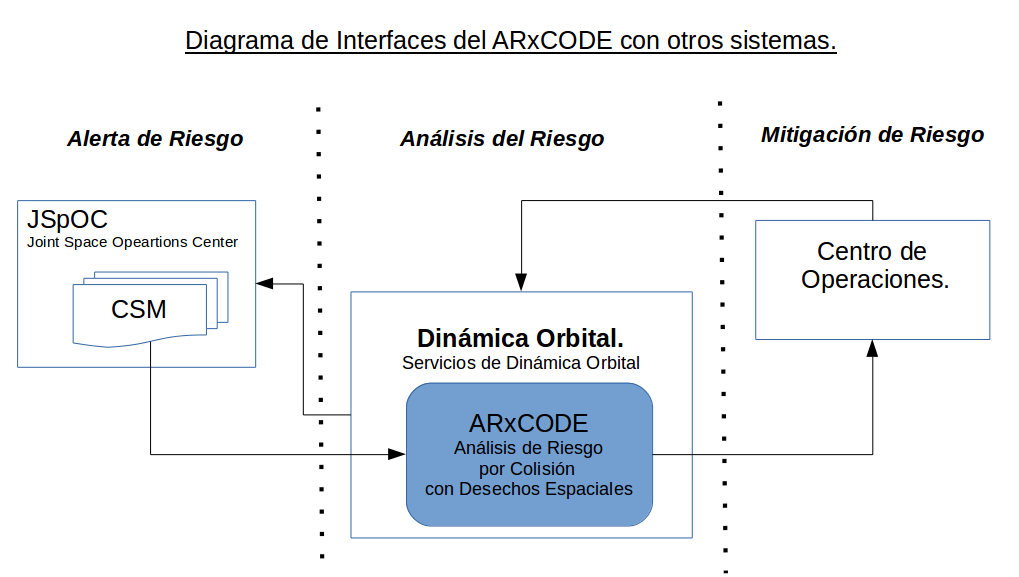
\includegraphics[width=0.8\textwidth]{imagenes/interfasessistemas}}
  \caption[Diagrama de Interfaces del Sistema]{Diagrama de Interfaces del Sistema}
  \label{fig:interfaces}
\end{figure}

No obstante, por cuestiones de tiempo y de accesibilidad, para el desarrollo de este trabajo, los datos que provee el departamento de Din\'amica Orbital fueron descargados y se extraen de un directorio, al igual que los mensajes de alerta CDM, que fueron descargados de p\'aginas de internet , ya que no nos han facilitado ninguno vinculado a la misi\'on operativa con la que trabajamos, por motivos de confidencialidad.\\
Se realiz\'o la automatizaci\'on de la descarga de TLEs de la p\'agina Space-Track y se habilit\'o en la interfaz la pantalla que permite la carga manual de los datos del encuentro.\\

En conclusi\'on, las interfaces implementadas, son:\\
 (Ver Fig. \ref{fig:interfacesImpl})\\
\begin{itemize}
\itemsep0em
 \item Conexi\'on a Space-Track para la solicitud de TLEs.
 \item Administraci\'on de las efem\'erides orbitales de los directorios de CodsAdmin.
 \item Administraci\'on de los CDM del directorio CDM, a trav\'es de la intervenci\'on del operador.
 \item Carga Manual de datos de un encuentro realizada por el operador.
\end{itemize}

\begin{figure}
\centering
  \fbox{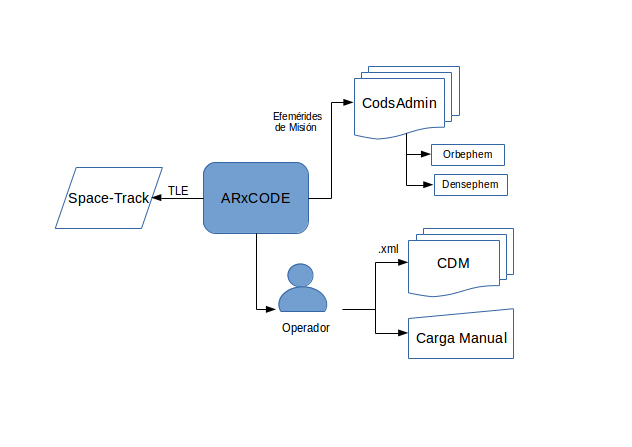
\includegraphics[width=0.8\textwidth]{imagenes/interfazImplementada}}
  \caption[Diagrama de Interfaces Implementadas en ARxCODE]{Diagrama de Interfaces Implementadas en ARxCODE}
  \label{fig:interfacesImpl}
\end{figure}

\section{Casos de Uso}

Este trabajo se pens\'o como un sistema acoplado al software principal del departamento de Din\'amica Orbital. En este sentido, no existe gran complejidad en la estructura del prototipo, ya que su valor, radica en la correcta implementaci\'on de los algoritmos que procesan la informaci\'on del encuentro. Identificamos dos casos de uso:\\
Fig. \ref{fig:casosuso}
 
 
\begin{itemize}
 \item {\it{Procesar Encuentro}}: que nuclea el procesamiento vertebral de ARxCODE
 \item {\it{Ver informes de encuentros anteriores}}: ofrece encuentros anteriores.
\end{itemize}

\begin{figure}[h]
  \centering
  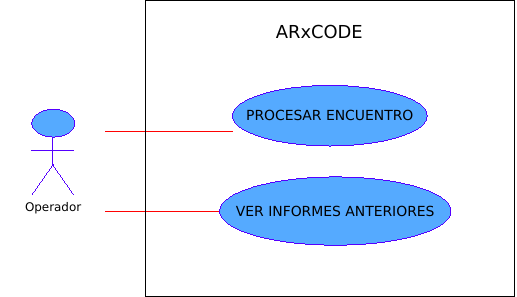
\includegraphics[width=.5\textwidth]{imagenes/usecaseAR}
  \caption{Casos de Uso de ARxCODE}
  \label{fig:casosuso}
\end{figure}


 \begin{table}[h]\renewcommand{\arraystretch}{1.3}
\centering
\resizebox{18cm}{!}{
\begin{tabular}[c]{|l|l|}
\hline 
\rowcolor{lightgray}
\bf{Nombre}  &    {\it{\bf{Procesar Encuentro}}}\\
\hline
Actor  &    Operador de Din\'amica Orbital con Autorizaci\'on\\
\hline
\multirow{ 3}{*}{Prop\'osito} & Calcular la probabilidad de colisi\'on, la m\'inima distancia total\\
& y m\'inima distancia en la coordenada radial, para poder hacer un an\'alisis\\
& de la situaci\'on de encuentro.\\
\hline
\multirow{ 4}{*}{Resumen}& Procesa la ingesta de datos de un encuentro, (CDMs o ingreso manual)\\
&  y calcula los par\'ametros de la situaci\'on de riesgo:\\
& m\'inima distancia total, m\'inima distancia en la coordenada radial y probabilidad de colisi\'on.\\
& Realiza gr\'aficos e informes.\\
\hline
\multirow{ 3}{*}{Precondiciones}  &  El operador debe estar registrado en la p\'agina space-track de NORAD.  \\
& Los archivos CDM deben estar previamente cargados en el Directorio de b\'usqueda.\\
& El operador debe conocer el encuentro que desea analizar y sus datos en caso del ingreso manual.\\
\hline
\multirow{ 3}{*}{Flujo Principal} & 1 - El operador selecciona un archivo CDM \\
& 2 - El operador oprime el bot\'on {\it{Track}} para visualizar el encuentro proyectado en la superficie terrestre (opcional)\\
& 3 - El operador oprime el bot\'on para generar un informe (opcional)\\
\hline
\multirow{ 3}{*}{Flujo Alternativo} & 1 - El operador ingresa los n\'umeros de identificaci\'on de los objetos (NORAD\_ID) \\
& 2 - El operador ingresa la fecha y hora del m\'aximo acercamiento (TCA)\\
& 3 - El operador oprime el bot\'on {\it{Procesar}} para procesar el encuentro\\
\hline
Postcondiciones & El informe de an\'alisis de riesgo fue generado y almacenado.\\
\hline
\end{tabular}}
\caption[Caso de Uso: Procesar Encuentro]{Tabla con la descripci\'on del caso de uso: \it{Procesar Encuentro}}
\label{tab:usoproceso}
\end{table}


\section{Arquitectura}

\subsection*{Componentes}\label{subsec:componentes}
En un planteo conceptual, con alto grado de abstracci\'on, los distintos paquetes de ARxCODE pueden agruparse en cinco componentes (Fig.  \ref{fig:componentes}): PROCESAMIENTO, ADMINISTRACI\'ON DE DATOS, INTERFAZ GR\'AFICA Y VISUALIZACI\'ON, Sistemas de Referencia y VALIDACIONES.\\

\begin{itemize}
 \item PROCESAMIENTO: Involucra los cuatro paquetes que, no s\'olo operan con los datos ingresados, sino que tambi\'en los manipulan y procesan para generar nuevos productos. Estos m\'odulos son, de alguna manera, los distintos n\'ucleos del c\'odigo.\\

 \begin{itemize}
 \itemsep0em
  \item {\it{AjustarTle}}
  \item {\it{Comparar}}
  \item {\it{Estadistica}}
  \item {\it{Encuentro}}
 \end{itemize}

 \item ADMINISTRACI\'ON DE DATOS: Son aquellos paquetes que se encargan de la obtenci\'on, el desglose y el preprocesamiento de los datos que ser\'an utilizados por el resto de los m\'odulos.

 \begin{itemize}
 \itemsep0em
  \item {\it{TleAdmin}}
  \item {\it{CodsAdmin}}
  \item {\it{CDM}}
 \end{itemize}

 \item INTERFAZ Y VISUALIZACI\'ON: Agrupa el paquete que genera la interfaz gr\'afica y el paquete que contiene todos los m\'odulos que generan representaciones visuales, como los gr\'aficos o las proyecciones de las trayectorias sobre el mapa.\\
 \begin{itemize}
 \itemsep0em
 \item {\it{Aplicacion}}
 \item {\it{visual}}
 \end{itemize}
 \item Sistemas de Referencia: {\it{SistReferencia}}, es el paquete que contiene todo lo referente a las transformaciones entre los distintos sistemas de referencia, ya sean espaciales o de tiempo.
 \item VALIDACIONES: Agrupa todos los m\'odulos desarrollados para validar los resultados.
\end{itemize}


\begin{figure}[h!]
  \centering
  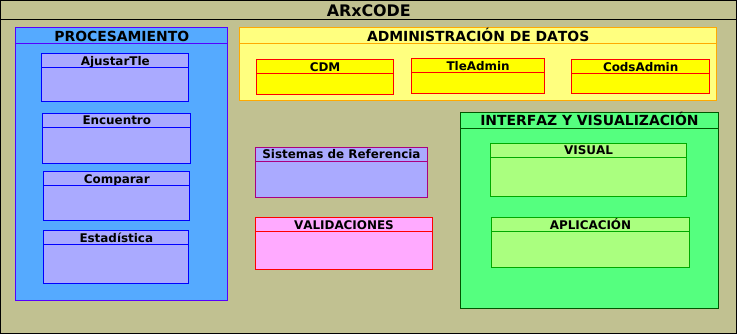
\includegraphics[width=.8\textwidth]{imagenes/componentesAR}  
  \caption{Componentes de ARxCODE}
  \label{fig:componentes}
\end{figure}

\subsubsection*{ADMINISTRACI\'ON DE DATOS: TleAdmin}
Este paquete contiene las dos clases que gestionan la descarga de los TLEs de la p\'agina Space-Track: {\bf{Tle}} y {\bf{setTLE}} (Fig. \ref{fig:Tleadmin}). La primera provee un \'unico TLE y todo lo referente a \'el; se instancia a partir del identificador de NORAD del objeto y una \'epoca, o a partir del nombre de un archivo que contiene un \'unico TLE. Entre sus m\'etodos, es fundamental {\bf{propagaTLE()}}, que propaga la posici\'on del objeto al momento que sea necesario.\\

La clase {\bf{setTLE}}, es necesaria particularmente para la implementaci\'on del m\'etodo de Osweiler que requiere un conjunto de TLEs de 15 d\'ias para la generaci\'on de la matriz de covarianza de la posici\'on del objeto. Esta clase se instancia, indicando el identificador de NORAD del objeto, la fecha de inicio y fin, del set que se requiere. Una vez descargados, genera un \'unico archivo con todos los TLEs del intervalo y los guarda en la carpeta {\it{crudosTLE}}.\\
El m\'etodo {\bf{divide\_setTLE()}} de la clase {\bf{setTLE}}, particiona el texto con el conjunto de TLEs y genera un archivo por cada TLE y lo almacena en la carpeta {\it{tle}} del paquete.\\
Esta \'ultima carpeta, se actualiza con cada corrida del software, de modo que siempre contiene s\'olo el conjunto de archivos de TLEs que van a ser procesados.\\

\begin{figure}[!h]
\centering
  \subfigure[Clase TLE (TleAdmin/TLE/Tle)]{
    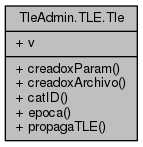
\includegraphics[width=0.3\textwidth]{imagenes/tleClass}
  }
  \hspace{1.5cm}
  \subfigure[Clase setTLE (TleAdmin/TLE/setTLE)]{
    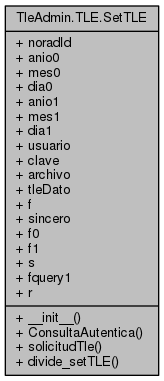
\includegraphics[width=0.3\columnwidth, keepaspectratio]{imagenes/setTLEclass}
  }
  \caption[Clases Tle y setTLE]{Clases Tle y setTLE del paquete TleAdmin}
  \label{fig:Tleadmin}
\end{figure}

\subsubsection*{ADMINISTRACI\'ON DE DATOS: CDM}
El paquete CDM contiene una carpeta con archivos en formato del CDM, en xml y la clase {\bf{CDM}} que tiene la capacidad de desglozarlos y extraer los datos del mensajes que ser\'an plasmados en la pantalla de la interfaz gr\'afica, para la visualizaci\'on del operador.\\

\subsubsection*{ADMINISTRACI\'ON DE DATOS: CodsAdmin}
Este paquete administra los productos orbitales generados por el departamento de Din\'amica Orbital \ac{CODS}.\\
Cuenta con varias carpetas que almacenan los productos previamente descargados y contiene a la clase {\bf{EphemCODS}}, que tiene la capacidad de extraer las efem\'erides de los archivos y de identificar el periodo de datos que abarca el archivo a partir del nombre.\\

\begin{figure}[!h]
\centering
  \subfigure[Clase CDM (CDM/CDM).]{
    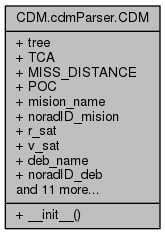
\includegraphics[width=.3\textwidth]{imagenes/cdmClass}
    \label{fig:clasetle}
  }
  \hspace{1.5cm}
  \subfigure[Clase EphemCODS (CodsAdmin/EphemCODS)]{
    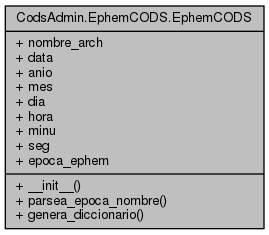
\includegraphics[width=0.4\columnwidth, keepaspectratio]{imagenes/ephemcodsClass}
    \label{fig:clasesettle}
  }
  \caption[Clases CDM y EphemCODS]{Clases CDM y EphemCODS para el pareseo de los mensajes de alerta CDM y los productos orbitales de \ac{CODS}}
\end{figure}

\subsubsection*{PROCESAMIENTO: AjustarTle}
Este paquete incluye el m\'odulo con el mismo nombre {\it{AjustarTle}}, que cuenta con varias funciones que reagrupan la informaci\'on del conjunto de TLEs a fin de poder hacer ordenamientos y comparaciones, entre los TLE de distintas fechas que son propagados a una misma \'epoca (pr\'actica necesaria para la implementaci\'on del m\'etodo de Osweiler para la construcci\'on de las matrices de covarianza).\\

\subsubsection*{PROCESAMIENTO: Comparar}
En el paquete {\it{Comparar}} se nuclean todos los m\'odulos y funciones que permiten la selecci\'on y la extracci\'on de los datos de los productos de Din\'amica Orbital (CODS), y sus respectivas comparaciones con los resultados que provienen de la propagaci\'on de los TLEs. Este tipo de comparaciones son necesarias en la estimaci\'on de errores que se comenten al utilizar propagaciones de los TLE con SGP4. 

\subsubsection*{PROCESAMIENTO: Estad\'istica}
Dentro de este paquete se encuentran los desarrollos referidos a los c\'alculos estad\'isticos, m\'as precisamente los m\'odulos que calculan las matrices de covarianza. En este paquete se encuentra el m\'odulo que implementa el m\'etodo de Osweiler {\bf{matrizOsweiler}}.

\subsubsection*{PROCESAMIENTO: Encuentro}
Este es el paquete n\'ucleo del software. En \'el se encuentra la clase {\bf{Encuentro}}  Fig. \ref{fig:claseencuentro}, que instancia la generaci\'on del encuentro, incorporando ambos objetos mediante sus identificadores de NORAD y el TCA, generando las propagaciones necesarias, y las matrices de error, para calcular la m\'inima distancia y la probabilidad de colisi\'on. A tal fin, cuenta con los m\'etodos (Fig. \ref{fig:claseencuentro}): {\bf{calculaMacombinada}}, {\bf{proyecta\_alplano\_encuentro}}, {\bf{calculaPoC\_circ}} y  {\bf{calculaPoC\_gral}}\\

\begin{figure}[h!]
  \centering
  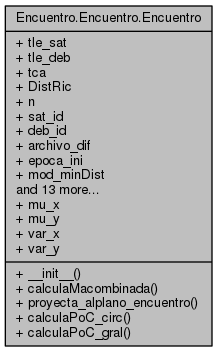
\includegraphics[width=.3\textwidth]{imagenes/encuentroClass} 
  \caption[Clase Encuentro]{Clase Encuentro para el c\'alculo de los par\'ametros del acercamiento}
  \label{fig:claseencuentro}
\end{figure}


\subsubsection*{INTERFAZ GR\'AFICA Y VISUALIZACI\'ON: Aplicaci\'on}
Este paquete contiene, principalmente el m\'odulo con el formulario de interfaz de ARxCODE {\bf{frm\_main}}. Dentro del mismo se ubican las clases que heredan de la estructura de QT, para el desarrollo de la aplicaci\'on, y son estas clases las que invocan los distintos m\'odulos del resto del c\'odigo para el desarrollo de los procesos.\\

\subsubsection*{INTERFAZ GR\'AFICA Y VISUALIZACI\'ON: visual}
{\bf{Visual}} es el paquete que agrupa todos los m\'odulos de generaci\'on de gr\'aficos y ploteos. Los gr\'aficos se utilizaron principalmente para el estudio de la tendencia de errores de los TLE y otros an\'alisis y validaciones.\\
Dentro de este paquete se encuentra el m\'odulo que genera las trayectorias de las \'orbitas, proyectadas sobre el mapa en el momento del encuentro.\\

\subsubsection*{Sistemas de Referencia}
Este paquete contiene m\'odulos para realizar transformaciones entre los distintos sistemas de referencia. Entre ellos, los dos m\'as utilizados son:
{\it{teme2tod}} y {\it{ricSis}}, ya descriptos en \ref{subsec:sistRef}.

\subsubsection*{Validaciones}
Re\'une todos los m\'odulos que se desarrollaron para la validaci\'on de los resultados, cuyos valores se analizan y publican en la secci\'on de Resultados y Validaciones Sec. \ref{chap:resultados}. A saber:

\begin{itemize}
 \item valida\_OSW: valida el m\'etodo de Osweiler.
 \item valida\_poc: valida los m\'etodos de c\'alculo de la probabilidad de colisi\'on.
 \item valida\_RTN: valida la transformaci\'on del sistema de referencia al RTN.
\end{itemize}


\section{Flujo din\'amico de ARxCODE}

ARxCODE se inicializa cuando un operador lo ejecuta.\\
Una vez iniciado el programa, el operador debe seleccionar alguna de las dos opciones de procesamiento: {\it{Cargar CDM}} o {\it{Carga Manual}}. Una vez cargados los datos se inicia la etapa del PROCESAMIENTO.\\

\subsection*{Procesamiento a partir de un CDM}
Si el procesamiento se realiza a partir de la carga de un CDM, el c\'odigo se ocupa de la extracci\'on y la publciaci\'on de los datos del CDM. 
\subsection*{Procesamiento a partir de una carga manual}
En el caso de la carga manual, el procesamiento implica distintos pasos Fig. \ref{fig:actdiag}:
\begin{itemize}
 \item Solicita los TLE a NORAD.
 \item Propaga los TLE y calcula el TCA y la m\'inima distancia.
 \item Calcula la covarianza del desecho, y de la misi\'on si la misma no fue provista por el departamento de Din\'amica Orbital.
 \item Calcula la matriz de covarianza combinada.
 \item Propaga la matriz de covarianza combinada hasta el TCA.
 \item Calcula la probabilidad de colisi\'on.
 \item Publica los datos en la pantalla para el operador.
\end{itemize}

Finalizada esta etapa de procesamiento y publicaci\'on de los datos por pantalla, el operador puede solicitar la visualizaci\'on de las trayectorias en el intervalo analizado, para ello presiona el bot\'on {\it{Track}} y el gr\'afico se agrega a la pantalla.\\

\begin{figure}[h!]
  \centering
  \fbox{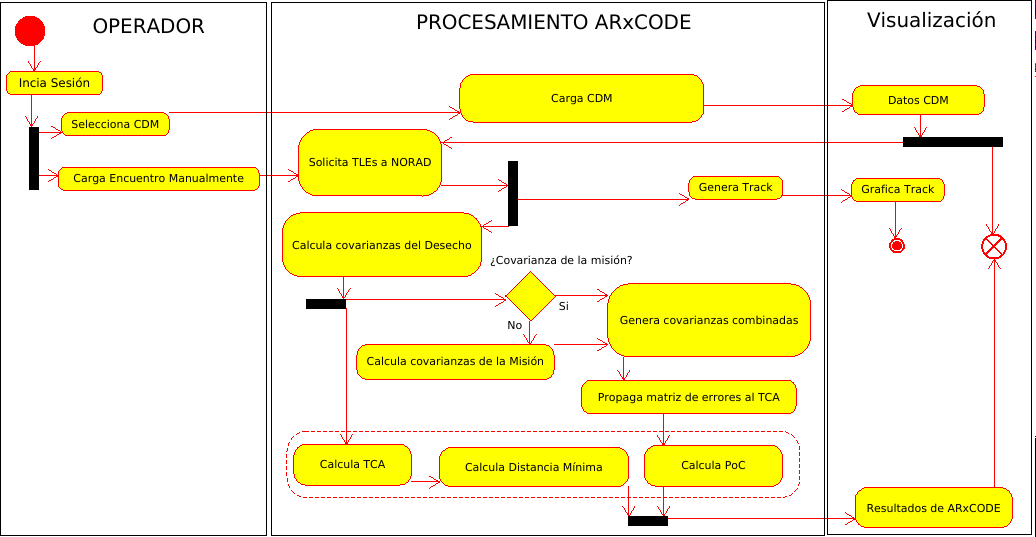
\includegraphics[width=\textwidth]{imagenes/actdiagAR}}
  \caption{Diagrama de Actividades de ARxCODE}
  \label{fig:actdiag}
\end{figure}

\subsection*{Pantallas del ARxCODE}


\begin{figure}[h!]
  \centering
  \fbox{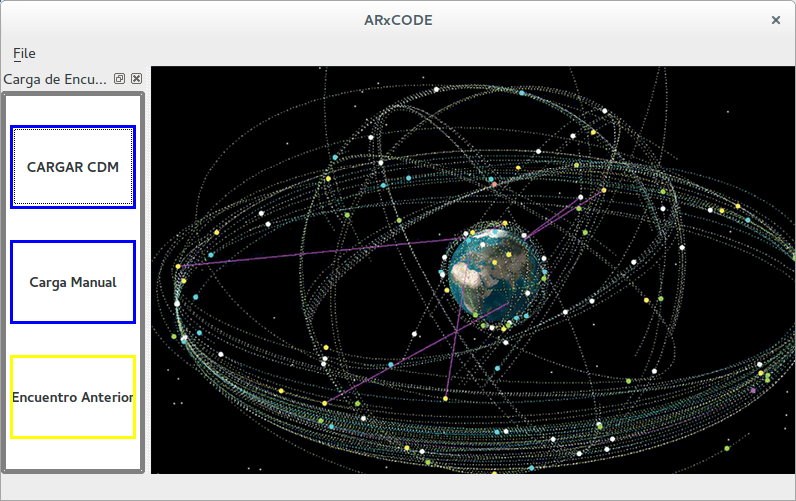
\includegraphics[width=0.8\textwidth]{imagenes/pantalla0}}
  \caption{Impresi\'on de la pantalla de inicio del ARxCODE}
  \label{fig:pantInicio}
\end{figure}

\begin{figure}[h!]
  \centering
  \fbox{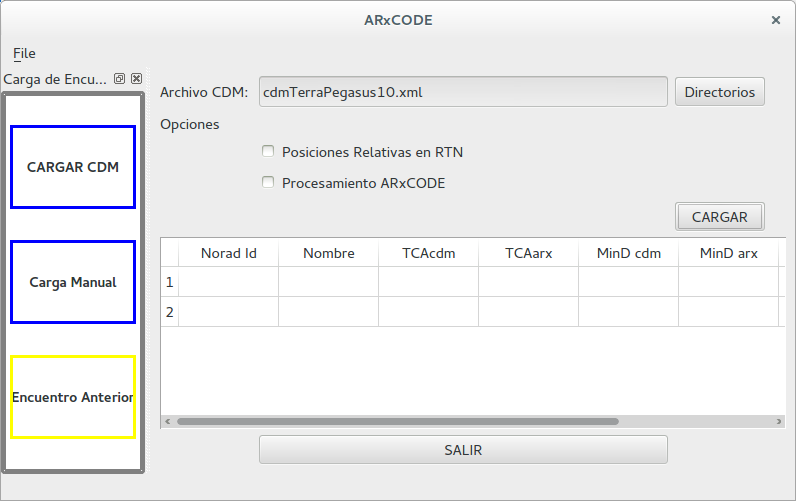
\includegraphics[width=0.8\textwidth]{imagenes/pantalla1}}
  \caption{Impresi\'on de la pantalla de Procesamiento de CDM del ARxCODE.}
  \label{fig:ingresadatosPant}
\end{figure}

\begin{figure}[h!]
  \centering
  \fbox{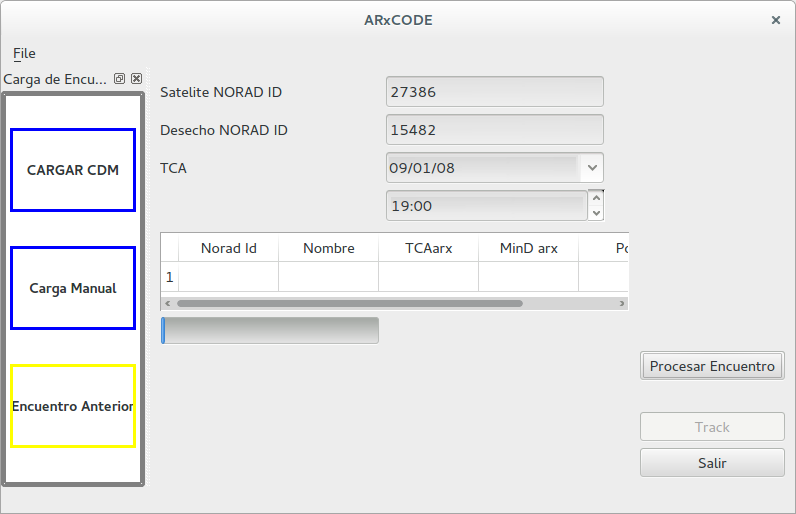
\includegraphics[width=0.8\textwidth]{imagenes/pantalla2}}
  \caption{Impresi\'on de la pantalla del ingreso manual de datos del ARxCODE}
  \label{fig:ingresadatosPant1}
\end{figure}

\begin{figure}[h!]
  \centering
  \fbox{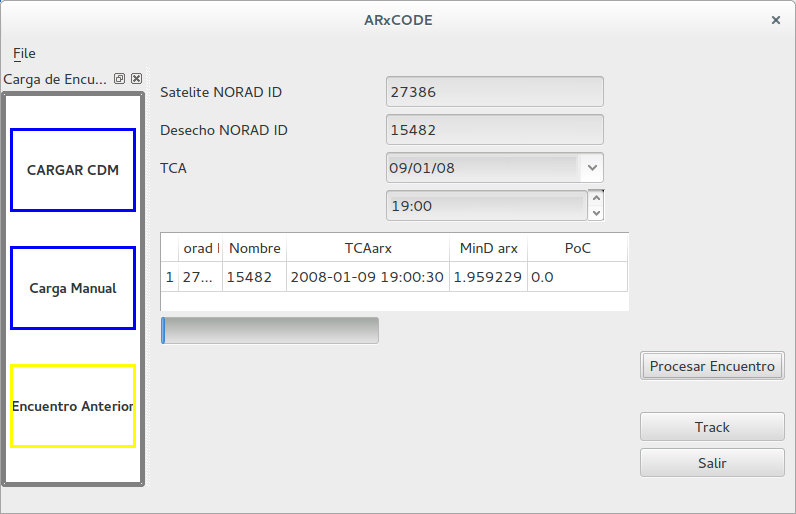
\includegraphics[width=0.8\textwidth]{imagenes/pantalla3}}
  \caption{Vista con la carga del procesamiento manual.}
  \label{fig:pantproc}
\end{figure}

\begin{figure}[h!]
  \centering
  \fbox{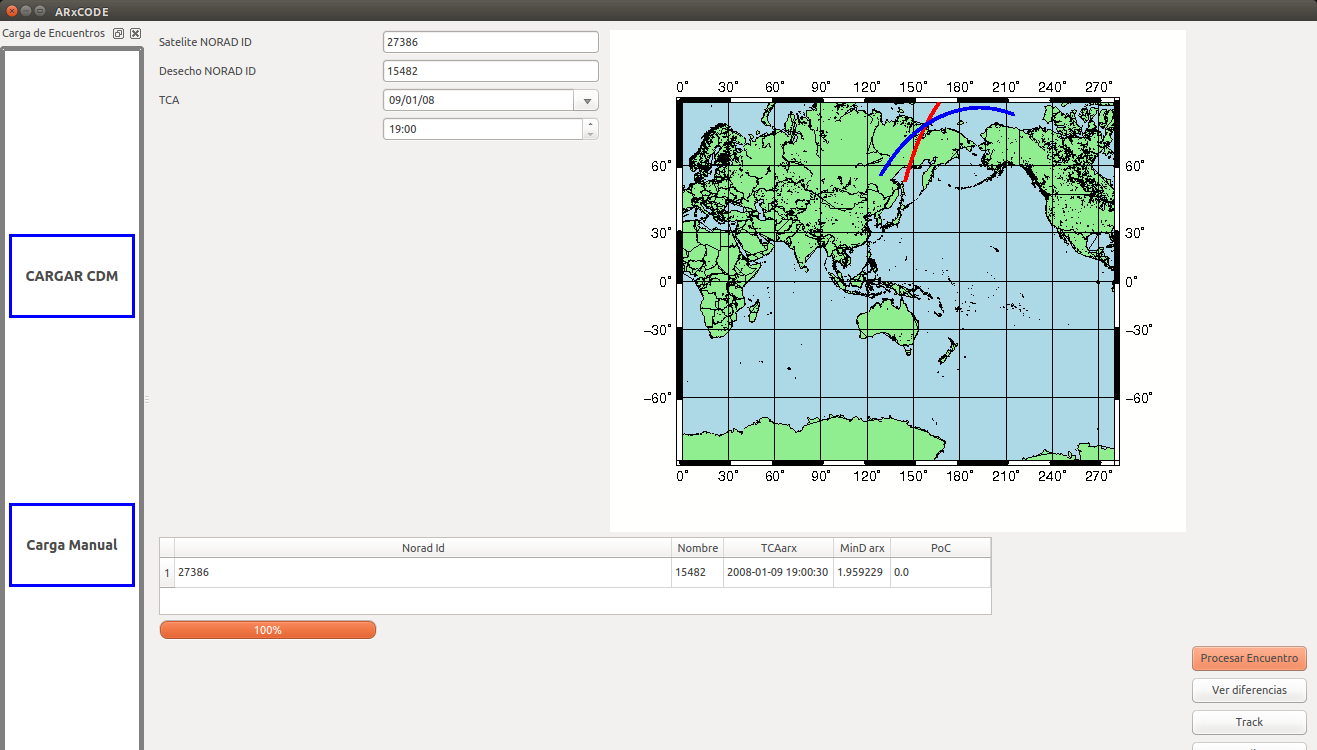
\includegraphics[width=0.8\textwidth]{imagenes/pantalla4}}
  \caption{Vista con los resultados publicados y la incorporaci\'on de las trayectorias.}
  \label{fig:pantfinal}
\end{figure}
% archivos y demases
% 
% \subsection*{Preprocesamiento de los Datos de Misi\'on de CODS}
% Para este trabajo CONAE nos facilit\'o el acceso a los datos orbitales de la misi\'on SAC-D.
% Los datos se ecuentran montados en un servidor que contiene la informaci\'on organizada en archivos con formato ASCII, distribuidos en distintas carpetas seg\'un su clasificaci\'on.\\
% Para la comparaci\'on que proponemos, solicitamos acceso a los archivos de efem\'erides orbitales ORBEPHEM, que ofrecen posiciones y velocidades tabuladas cada un minuto, en el Sistema de Referencia TOD (True of Date), en coordenadas cartesianas.
% 
% \subsection*{ORBEPHEM}
% Estos productos son generados luego de un post procesamiento que incluye una propagaci\'on ajustada por una determinaci\'on orbital. 
% Cada archivo contiene un listado cronol\'ogicamente tabulado de posiciones y velocidades, dentro de un periodo de casi 3 d\'ias. ( doc\_interfaces)
% 
% La nomenclatura de los mismos respeta el siguiente formato:\\
% \begin{verbatim}
%  CODS_YYYYMMDD_HHMMSS_SACD_ORBEPHEM_TOD_XYZ_O.TXT
%  
%  Donde:
%   CODS = Identifica el Servicio dentro del CUSS que presta la información.
%   YYYYMMDD_HHMMSS = epoca de generación del dato.
%   SACD = Identificación del Satélite.
%   ORBEPHEM = Tipo de Dato, Efeméride Orbital (procesada a posteriori)
%   TOD = Sistema de Referencia True of Date.
%   XYZ = Tipo de efeméride, cartesiana.
%   O = Operacional. 
% \end{verbatim}


% \subsection*{Archivos Utilizados}
% Si bien la nomenclatura de los archivos respeta una estructura, s\'olo se indica en el nombre, la fecha de generaci\'on de los datos y no puede desprenderse del mismo cu\'al es la \'epoca final e inicial de cada archivo, y no existe un registro del los gaps de datos ausentes. A su vez, las \'epocas contempladas en cada uno de ellos no está homogeneizada. Es decir, la fecha y hora inicial y final de cada registro es diferente para cada archivo.\\
% Dada esta organizaci\'on, para el punto tres del procedimiento, referente a la localizaci\'on del archivo necesario para la comparaci\'on, la b\'usqueda se realiza de la siguiente manera:\\
% Localizamos en primer lugar el archivo cuyo nombre coincide con la fecha de la \'epoca del TLE primario.
% Como una misma fecha se encuentra en m\'as de un archivo, buscamos el archivo que contenga esa fecha y que adem\'as sea el m\'as actualizado de todos. Para ello, además del archivo cuyo nombre contiene la fecha del TLE primario, se enlistan los siguientes dos archivos y se ordenan en orden decreciente, de manera que el primer lugar de la lista lo ocupe el \'ultimo de los archivos seleccionados. Finalmente se comienza el proceso iterativo de abrir los archivos, evaluar el contenido y ver si se encuentran los dos registros que encierren la \'epoca del TLE.
% Una vez que se encuentran las l\'ineas de efem\'erides que contienen la \'epoca de inter\'es se interpola, y se termina la iteraci\'on.
% 
% \noindent
% Cantidad TOTAL de archivos $=  1454$\\
% Cantidad media de resgistros por archivo $=  2688$\\
% Archivo con el mayor n\'umero de registros $=  3042$\\
% Archivo con el menor n\'umero de registros $=  142$\\

